%! TeX program = lualatex
\documentclass[a4paper,11pt]{article} 
% packages
\usepackage{censor}
\StopCensoring
\usepackage{fontspec}
\setmainfont{EB Garamond}
% for tironian et fallback
% % \directlua{luaotfload.add_fallback
% % ("emojifallback",
% %      {"Noto Serif:mode=harf"}
% % )}
% % \setmainfont{EB Garamond}[RawFeature={fallback=emojifallback}]

\setmonofont[Scale=MatchLowercase]{Deja Vu Sans Mono}
\usepackage[a4paper,left=2cm,right=2cm,top=\dimexpr15mm+1.5\baselineskip,bottom=2cm]{geometry}
\setlength{\parindent}{0pt}

\usepackage{fancyhdr}       % Headers and footers 
\fancyhead[R]{\normalfont \leftmark}
\fancyhead[L]{}
\pagestyle{fancy}

\usepackage{microtype}      % Slightly tweak font spacing for aesthetics
\usepackage{multicol}
\usepackage[english]{babel} % Language hyphenation and typographical rules
\usepackage{xcolor}
\definecolor{linkblue}{RGB}{0, 64, 128}
\usepackage[final, colorlinks = false, urlcolor = linkblue]{hyperref} 
% \newcommand{\secref}[1]{\textbf{§~\nameref{#1}}}
\newcommand{\secref}[1]{\textbf{§\ref{#1}~\nameref{#1}}}

\usepackage{changepage}     % adjust margins on the fly

\usepackage{minted}
\usemintedstyle{algol_nu}

\usepackage{pgfplots}
\pgfplotsset{width=\textwidth,compat=1.9}

\usepackage{caption}
\newenvironment{code}{\captionsetup{type=listing}}{}
\captionsetup[listing]{skip=0pt}
\setlength{\abovecaptionskip}{5pt}
\setlength{\belowcaptionskip}{5pt}

\usepackage[yyyymmdd]{datetime}
\renewcommand{\dateseparator}{--}

\usepackage{enumitem}

\usepackage{titlesec}

\author{Andrew Hayes}

\begin{document}
\begin{titlepage}
    \begin{center}
        \hrule
        \vspace*{0.6cm}
        \censor{\huge \textbf{CT436}}
        \vspace*{0.6cm}
        \hrule
        \LARGE
        \vspace{0.5cm}
            Advanced Professional Skills
        \vspace{0.5cm}
        \hrule

        \vfill
        \vfill

        \hrule
        \begin{minipage}{0.495\textwidth} 
            \vspace{0.4em}
            \raggedright
            \normalsize 
            Name: Andrew Hayes \\
            E-mail: \href{mailto://a.hayes18@universityofgalway.ie}{\texttt{a.hayes18@universityofgalway.ie}}  \hfill\\   
            Student ID: 21321503 \hfill
        \end{minipage}
        \begin{minipage}{0.495\textwidth} 
            \raggedleft
            \vspace*{0.8cm}
            \Large
            \today
            \vspace*{0.6cm}
        \end{minipage}
        \medskip\hrule 
    \end{center}
\end{titlepage}

\pagenumbering{roman}
\newpage
\tableofcontents
\newpage
\setcounter{page}{1}
\pagenumbering{arabic}

\section{Introduction}
\subsection{Lecturer Contact Information}
\begin{itemize}
    \item   Dr. Owen Molloy (\href{mailto://owen.molloy@universityofgalway.ie}{\texttt{owen.molloy@universityofgalway.ie}}
\end{itemize}

\subsection{Group Project}
\begin{itemize}
    \item   Groups of 3 -- 5.
    \item   Work on an idea that your team is excited about.
    \item   Take the ideation \& team formation phase very seriously: it can greatly determine your experience
            within the class.
    \item   If you find that your idea hits a dead-end, do not be afraid to pivot mid-way through the semester.
\end{itemize}

Each team will maintain an online portfolio documenting their journey \& linking with or containing their deliverables:
\begin{multicols}{2}
\begin{itemize}
    \item   Idea generation.
    \item   Market segmentation / analysis.
    \item   End-user profiling.
    \item   Customer persona.
    \item   Lifecycle use case.
    \item   Quantified value proposition.
    \item   Product brochure.
    \item   Business model canvas / business plan.
    \item   Video (which will be submitted to EI Student Entrepreneur Awards).
\end{itemize}
\end{multicols}

\section{Innovation}
\textbf{Innovation} consists of using new technology \& new ways of thinking to add value to an existing idea or
product and to make substantial changes in society.
Innovation = Invention $\times$ Commercialisation.

\subsection{Four Misinterpretations of Innovation}
\begin{enumerate}
    \item   \textbf{Innovation $\neq$ Invention}: An invention is a creative idea while an innovation makes that idea 
            feasible and turns it into a product or service that satisfies the customer's needs.

    \item   \textbf{Innovation $\neq$ New Products and/or Services}: Innovation has rightly been associated with many 
            cases of new product development.
            However, innovation can concern other new developments such as new markets or new marketing methods.

    \item   \textbf{Innovation $\neq$ Original}: Innovation often builds on old existing ideas \& resources.
    
    \item   \textbf{Innovation $\neq$ One-Off Inspiration}: Unlike the one sudden flash of inspiration, innovation
            is a gradual process that takes place over a period of time (or incubation).
\end{enumerate}

\subsection{Sources of Innovation}
Innovators are generally attentive to changes which give them clues to what opportunities may come in future.
Would-be innovators must also go out and look, ask, \& listen.
Above all, innovation is \textit{work} rather than \textit{genius}.
It requires knowledge, it requires focus, and it often requires integrity.

\begin{figure}[H]
    \centering
    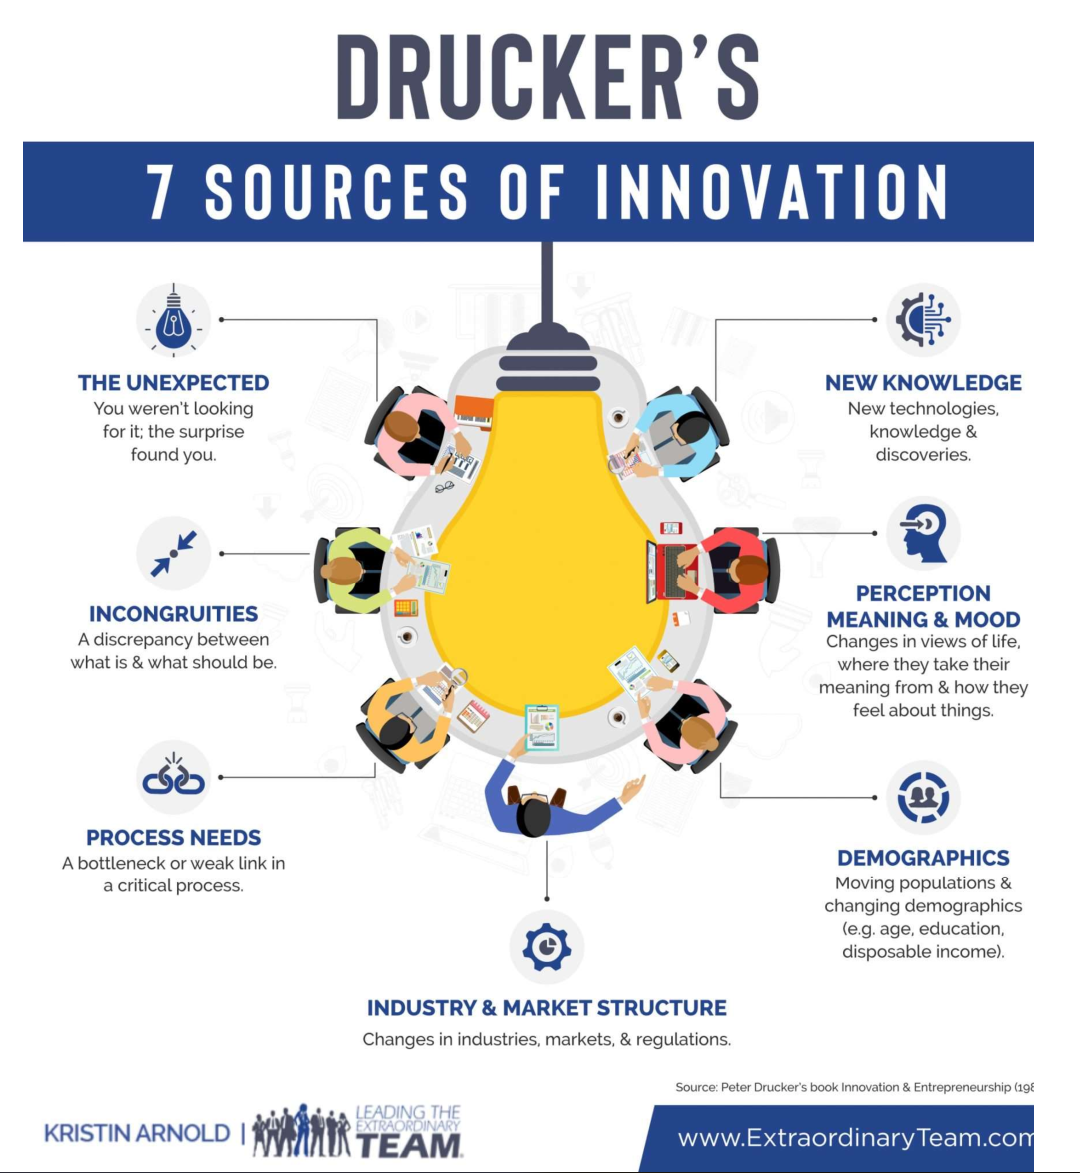
\includegraphics[width=0.6\textwidth]{images/druckers_sources_of_innovation.png}
    \caption{Drucker's Sources of Innovation}
\end{figure}

\subsection{Types of Innovation}
\begin{itemize}
    \item   \textbf{Invention:} Totally new product, service, or process.
    \item   \textbf{Extension:} New use or different application of an already existing product, service, or process.
    \item   \textbf{Duplication:} Creative replication of an existing concept.
    \item   \textbf{Synthesis:} Combination of existing concepts \& factors into a new formulation or use.
\end{itemize}

\section{Entrepreneurship}
\textbf{Entrepreneurship} is the formation of a new venture that produces a product or offering that creates some value to 
make it economically sustainable.
It has the ability to improve standards of living \& create wealth.
\\\\
In contemporary markets, entrepreneurs act as innovators or developers who identify \& capture opportunities, transform 
the opportunities into merchandisable concepts, create value through multiple stakeholders \& resources, and take risks 
while seeking rewards for their ventures \& efforts.

\subsection{What do you need to start a successful new venture?}
\begin{enumerate}
    \item   Idea.
    \item   Team.
    \item   Process.
\end{enumerate}

Good entrepreneurial business ideas are:
\begin{enumerate}
    \item   \textbf{Market-Driven:}
            \begin{itemize}
                \item   Solve a problem.
                \item   Find a market need.
                \item   Customer-focused, not product-driven.
                \item   Targets an identified sizeable market segment.
            \end{itemize}
    \item   \textbf{Feasible:}
            \begin{itemize}
                \item   Attractive: there is a demand.
                \item   Achievable: it can be done.
                \item   Durable: it lasts.
                \item   Value-Creating: it is worth something.
                \item   Safe.
                \item   Affordable.
            \end{itemize}
    \item   \textbf{Unique:}
            \begin{itemize}
                \item   Faster/Better/Cheaper.
                \item   Differentiated (vs. commodity).
            \end{itemize}
    \item   \textbf{Fundable:}
            \begin{itemize}
                \item   Revenue stream.
                \item   Management risk.
                \item   Sustainable: market exists with frequency of purchase.
                \item   Scaleable or replicable.
                \item   Barriers to entry.
                \item   Growth potential.
                \item   Product pipeline.
                \item   Exit plan.
                \item   Innovative.
            \end{itemize}
    \item   \textbf{Innovative:}
            \begin{itemize}
                \item   Invention: totally new product/service/process.
                \item   Extension: new use or different application of an already existing product/service/process.
                \item   Duplication: creating a replication of an existing concept.
                \item   Synthesis: combining existing concepts and/or factors into new formula for use.
            \end{itemize}
\end{enumerate}








\end{document}
